\documentclass[a4paper,12pt,oneside]{report} % nie: report!


% pakiety
\usepackage{polski} % lepiej to zamiast babel!
\usepackage[utf8]{inputenc} % w razie kłopotów spróbować: \usepackage[utf8x]{inputenc}
\usepackage{fancyhdr} % nagłówki i stopki
\usepackage{indentfirst} % WAŻNE, MA BYĆ!
\usepackage[pdftex]{graphicx} % to do wstawiania rysunków
\usepackage{amsmath} % to do dodatkowych symboli, przydatne
\usepackage[pdftex,
            left=1in,right=1in,
            top=1in,bottom=1in]{geometry} % marginsy
\usepackage{amssymb} % to też do dodatkowych symboli, też przydatne
\usepackage{pdfpages}
\usepackage{lipsum}
\usepackage{multirow}
\usepackage{listings}
\usepackage{caption}
\usepackage{booktabs}
\usepackage{subcaption}
\usepackage{xcolor}
\graphicspath{ {./pics/} }

% definicje nagłówków i stopek
\pagestyle{fancy}
\renewcommand{\chaptermark}[1]{\markboth{#1}{}}
\renewcommand{\sectionmark}[1]{\markright{\thesection\ #1}}
\fancyhf{}
\fancyhead[LO]{\footnotesize\rightmark}
\renewcommand{\headrulewidth}{0.5pt}
\renewcommand{\footrulewidth}{0pt}
\addtolength{\headheight}{1.5pt}
\fancypagestyle{plain}{\fancyhead{}\cfoot{\footnotesize\bfseries\thepage}\renewcommand{\headrulewidth}{0pt}}


% interlinia
\linespread{1.25}

\title{Instalacja PHP z źródeł }
\author{Aleh Hutsko}

% treść
\begin{document}

\maketitle


\tableofcontents{}
\chapter{Opis programu}

PHP – interpretowany, skryptowy język programowania zaprojektowany do generowania stron internetowych i budowania aplikacji webowych w czasie rzeczywistym.

PHP jest najczęściej stosowany do tworzenia skryptów po stronie serwera WWW, ale może być on również używany do przetwarzania danych z poziomu wiersza poleceń, a nawet do pisania programów pracujących w trybie graficznym (np. za pomocą biblioteki GTK+, używając rozszerzenia PHP-GTK). Implementacja PHP wraz z serwerem WWW Apache oraz serwerem baz danych MySQL określana jest jako platforma AMP (w środowisku Linux – LAMP, w Windows – WAMP).

\chapter{Przebieg procesu instalacji oprogramowania}
\section{Instalacja zależności, pobranie "source code", rozpakowanie paczki}

Poniższe kroki opisują \textit{Rysunek \ref{fig:first}}:

\begin{enumerate}
    \item Pierwszym krokiem była instalacja zależności. Ponieważ robiłem to wcześniej, nowych instalacji paczek nie ma. \\ \textbf{sudo apt install} \textit{...}
    \begin{itemize}
        \item pkg-config
        \item build-essential
        \item autoconf
        \item bison
        \item re2c
        \item libxml2-dev
        \item libsqlite3-dev
    \end{itemize}
    \item drugim krokiem było pobranie "source code". \\ \textbf{wget https://github.com/php/php-src/archive/refs/tags/php-8.0.20.tar.gz}
    \item sprawdziłem czy się pobrało (okazało się udano),stworzyłem katalog \textit{~/build/php/8.0.20/} skopiowałem ten plik do katalogu  \\ \textbf{cp php-8.0.20.tar.gz build/php/8.0.20/}
    \item Rozpakowałem paczkę za pomocą komendy: \\ \textbf{ tar -zxvf php-8.0.20.tar.gz}
\end{enumerate}

\begin{figure}[hb]
    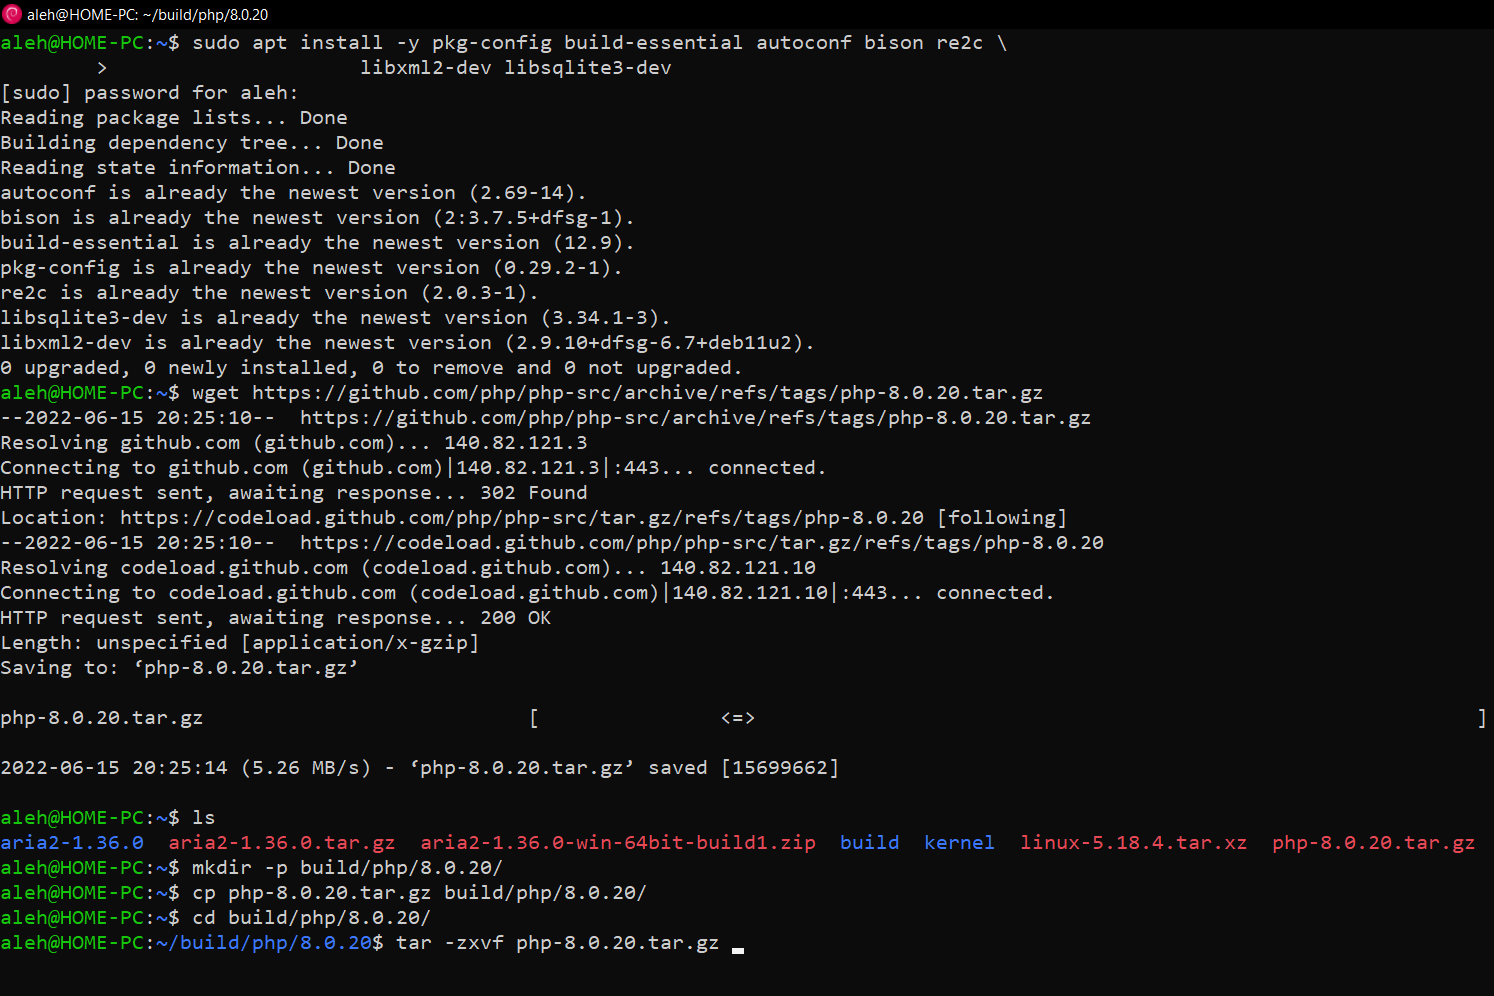
\includegraphics[width=16cm]{e6.png}
	\caption{Instalacja zależnosci, pobranie "source code", Rozpakowanie archiwum }
    \label{fig:first}
\end{figure}


\section{Koniec rozpakowania, utworzenie konfiguracji, konfiguracja buildu, make}

Domyślnie w kodzie źródłowym PHP nie ma pliku konfiguracji, i trzeba go utworzyć.

Poniższe kroki opisują \textit{Rysunki \ref{fig:second} -- \ref{fig:fourth}}:

\begin{enumerate}
    \item Przechodze do rozpakowanego katalogu \\ \textbf{cd php-src-php-8.0.20/}
    \item Próbuję stworzyć plik konfiguracji za pomocą wywoływania scryptu \textit{"./buildconf"}, ale występuje błąd i polecane wywołać polecenie (Rysunek \ref{fig:second}) \\ \textbf{./buildconf -{}-force}
    \item Po utworzeniu konfiguracji robię konfiguracje buildu :) (Rysunek \ref{fig:third})  \\ \textbf{ ./configure -{}-enable-debug}
    \item Po konfiguracji sprawdziłem rdzeni (polecenie \textbf{nproc}), i później robię polecenie make  (Rysunek \ref{fig:fourth}) \\ \textbf{ make -j4}
\end{enumerate}

\begin{figure}[h]
    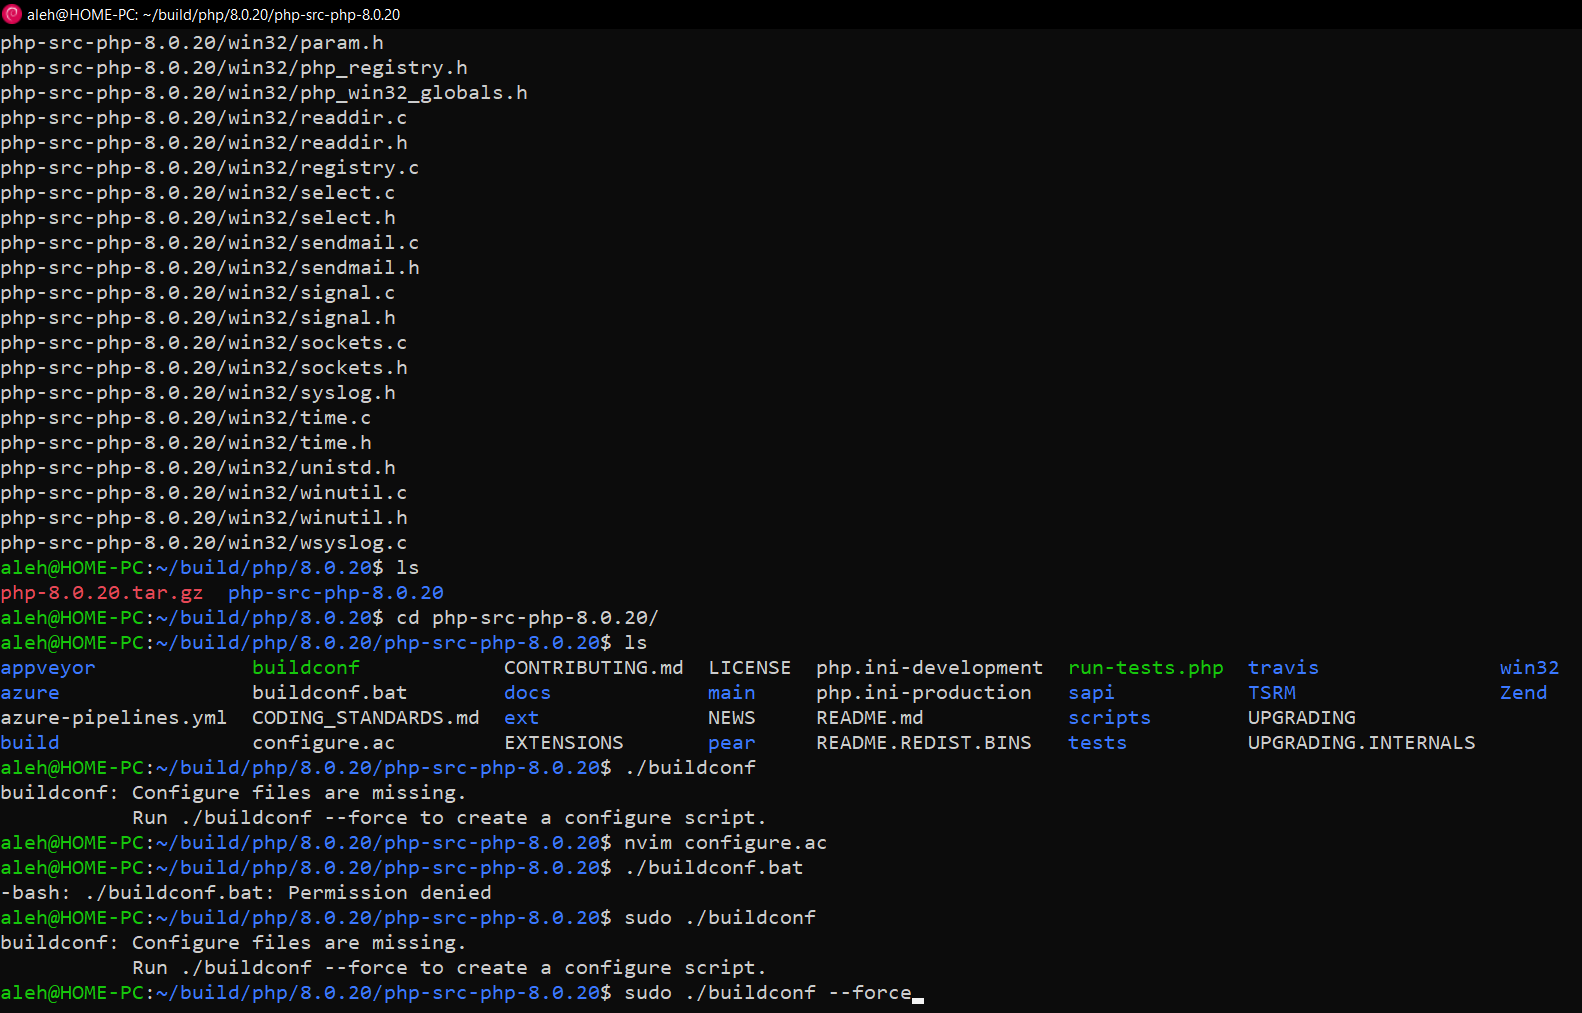
\includegraphics[width=16cm]{e7.png}
	\caption{Koniec rozpakowania, utworzenie konfiguracji}
    \label{fig:second}
\end{figure}


\begin{figure}[h]
    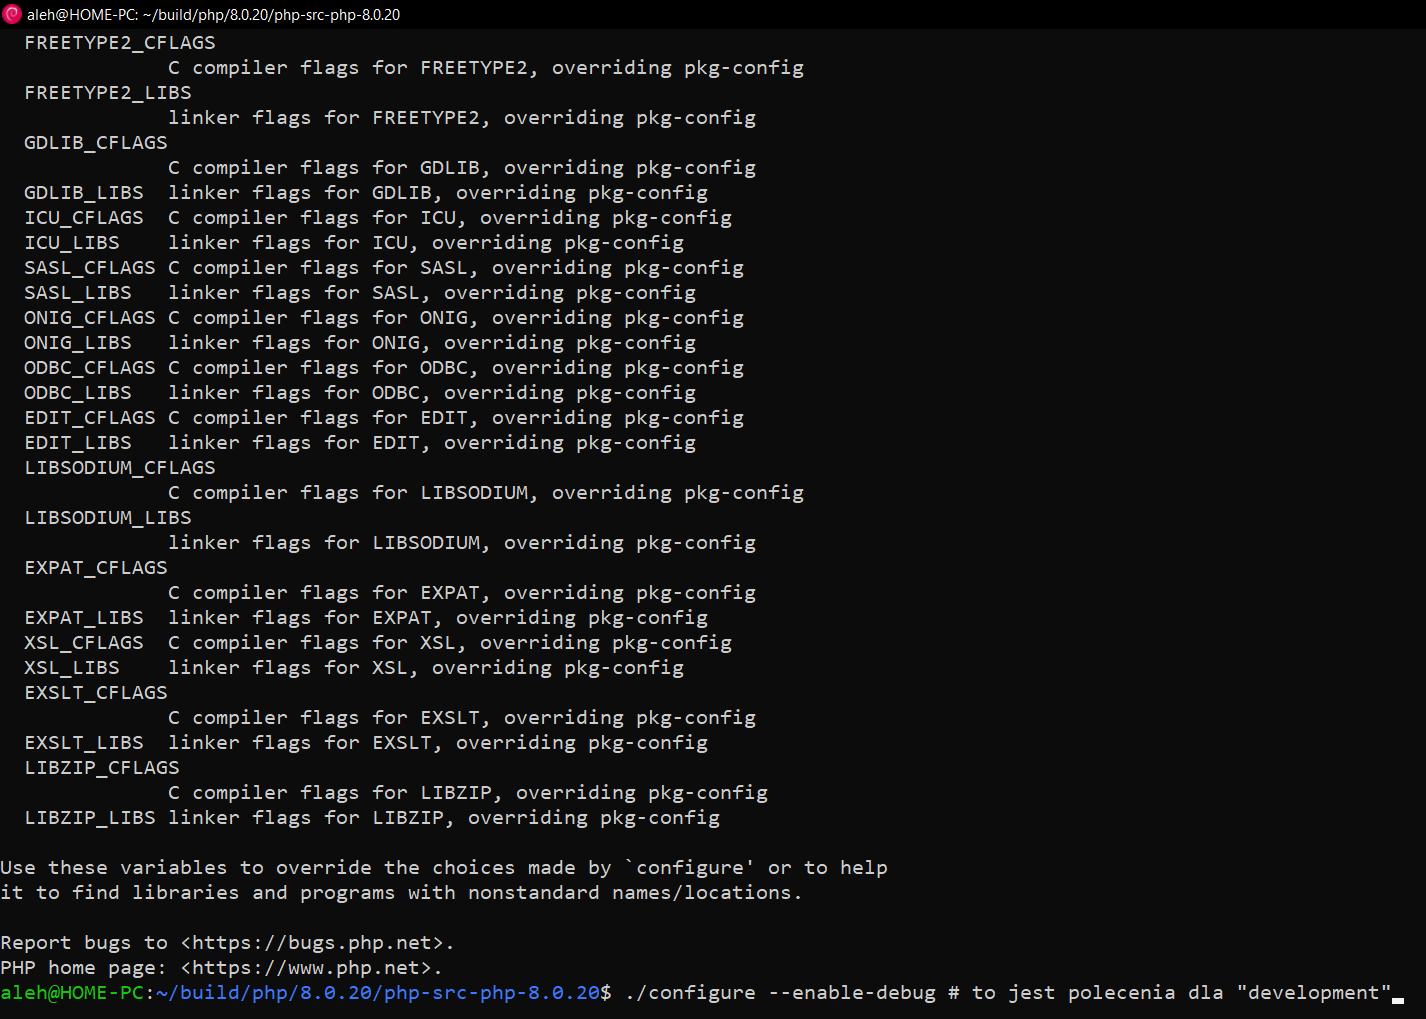
\includegraphics[width=16cm]{e8.png}
	\caption{Konfiguracja buildu}
    \label{fig:third}
\end{figure}

\begin{figure}[h]
    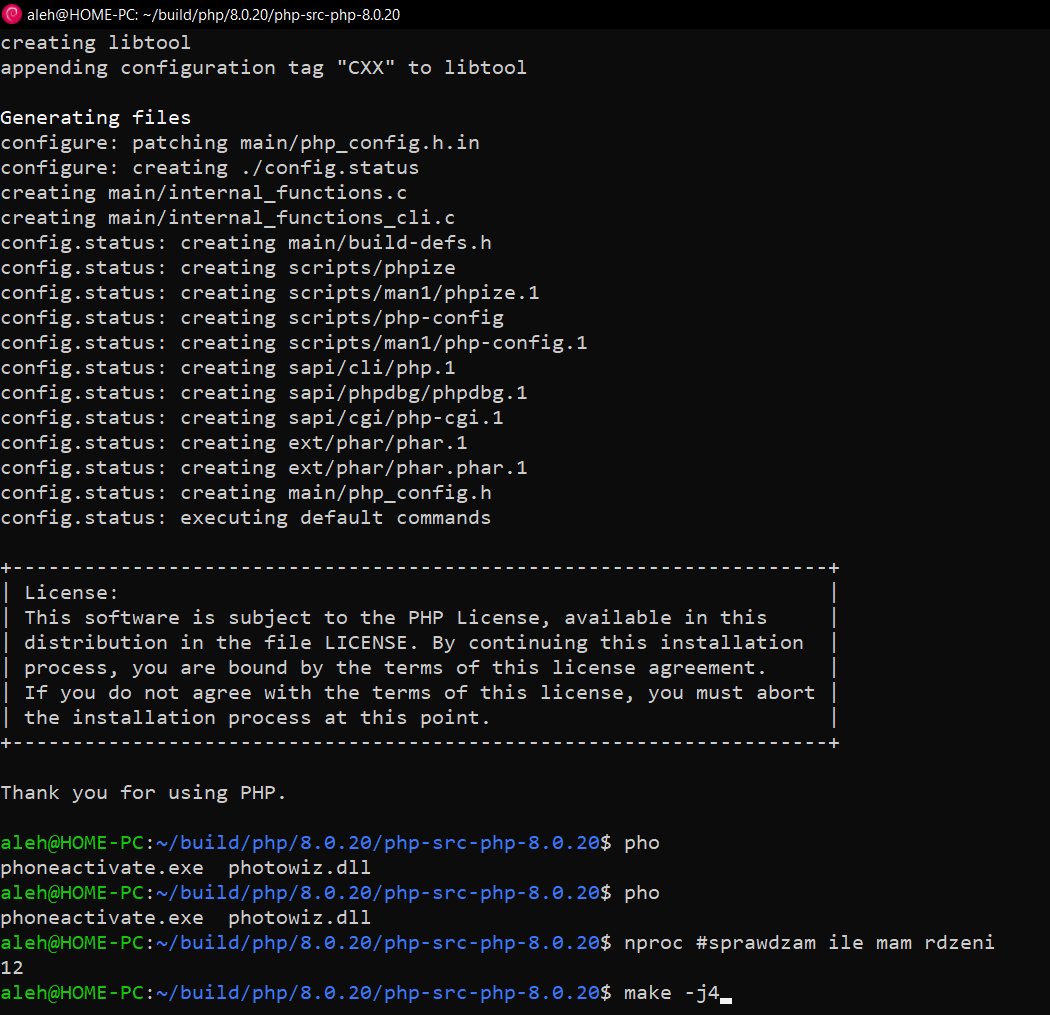
\includegraphics[width=16cm]{e9.png}
	\caption{Koniec konfiguracji buildu, polecenie "make"}
    \label{fig:fourth}
\end{figure}


\section{make test, make install}


\begin{enumerate}
    \item Robię polecenie testowania (po którym został wykryty jakiś błąd i pytanie, czy można wyśłać logi, wysłałem) \textit{(Rysunek \ref{fig:fifth})} \\ \textbf{make test}
    \item Próbuję wykonać \textit{make install}, prompt pisze, że nie ma uprawnień \textit{(eng. Permission denied)}, więc dodaje \textit{sudo} \textit{(Rysunek \ref{fig:sixth})} \\ \textbf{sudo make install}
    \item I w końcu sprawdzam sobie, czy PHP został zainstalowany. Na początku wpisuje \textbf{ph} i klikam [TAB], później \textbf{php -a}. \textit{(Rysunek \ref{fig:seventh})}
\end{enumerate}

\begin{figure}[h]
    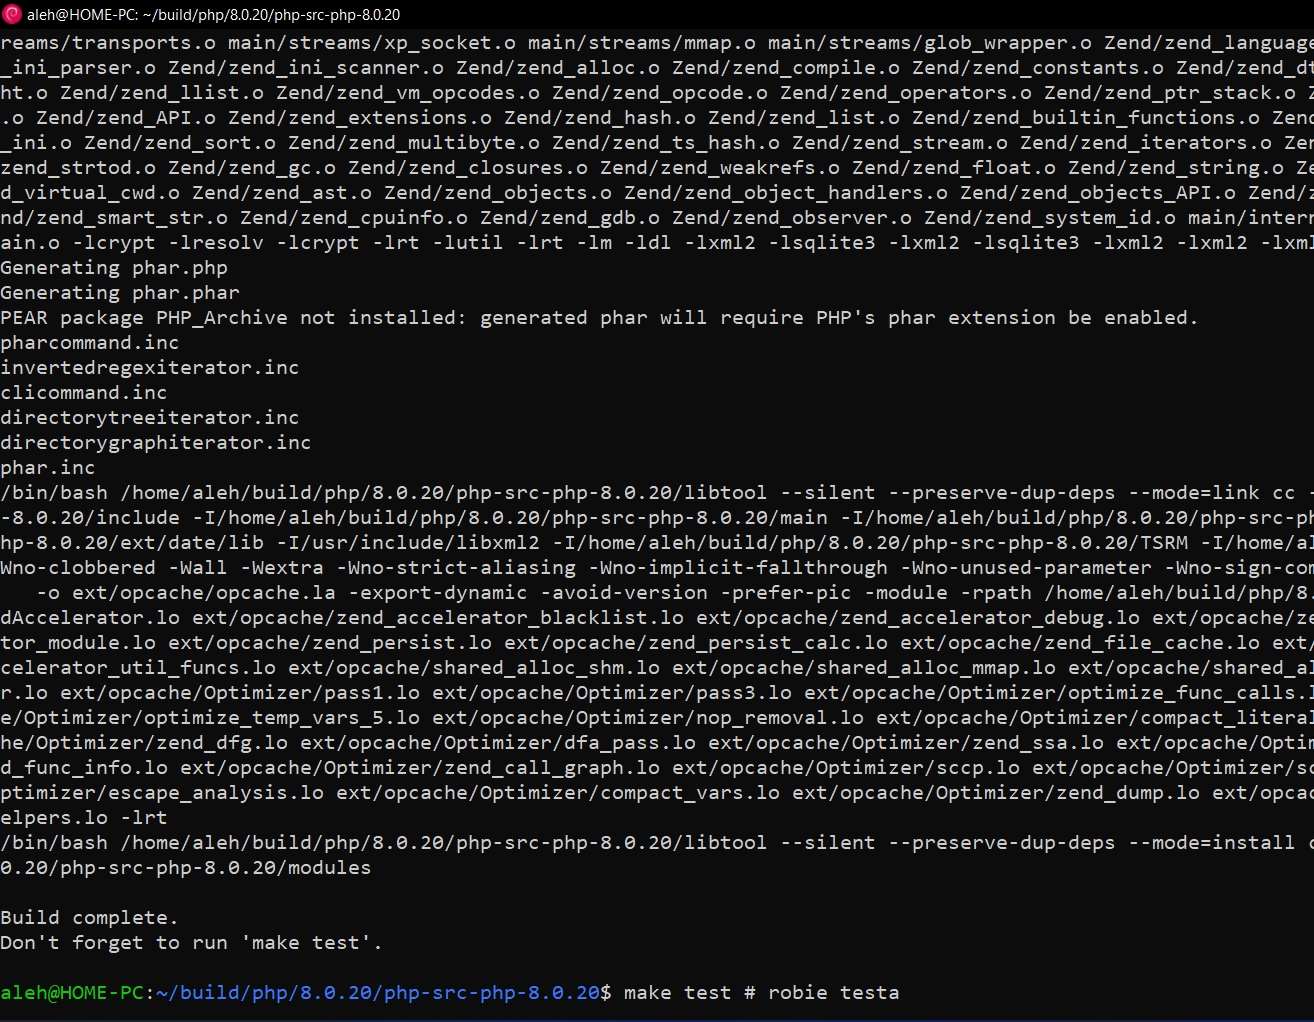
\includegraphics[width=16cm]{e10.png}
	\caption{Koniec "make", polecenie "make test"}
    \label{fig:fifth}
\end{figure}

\begin{figure}[h]
    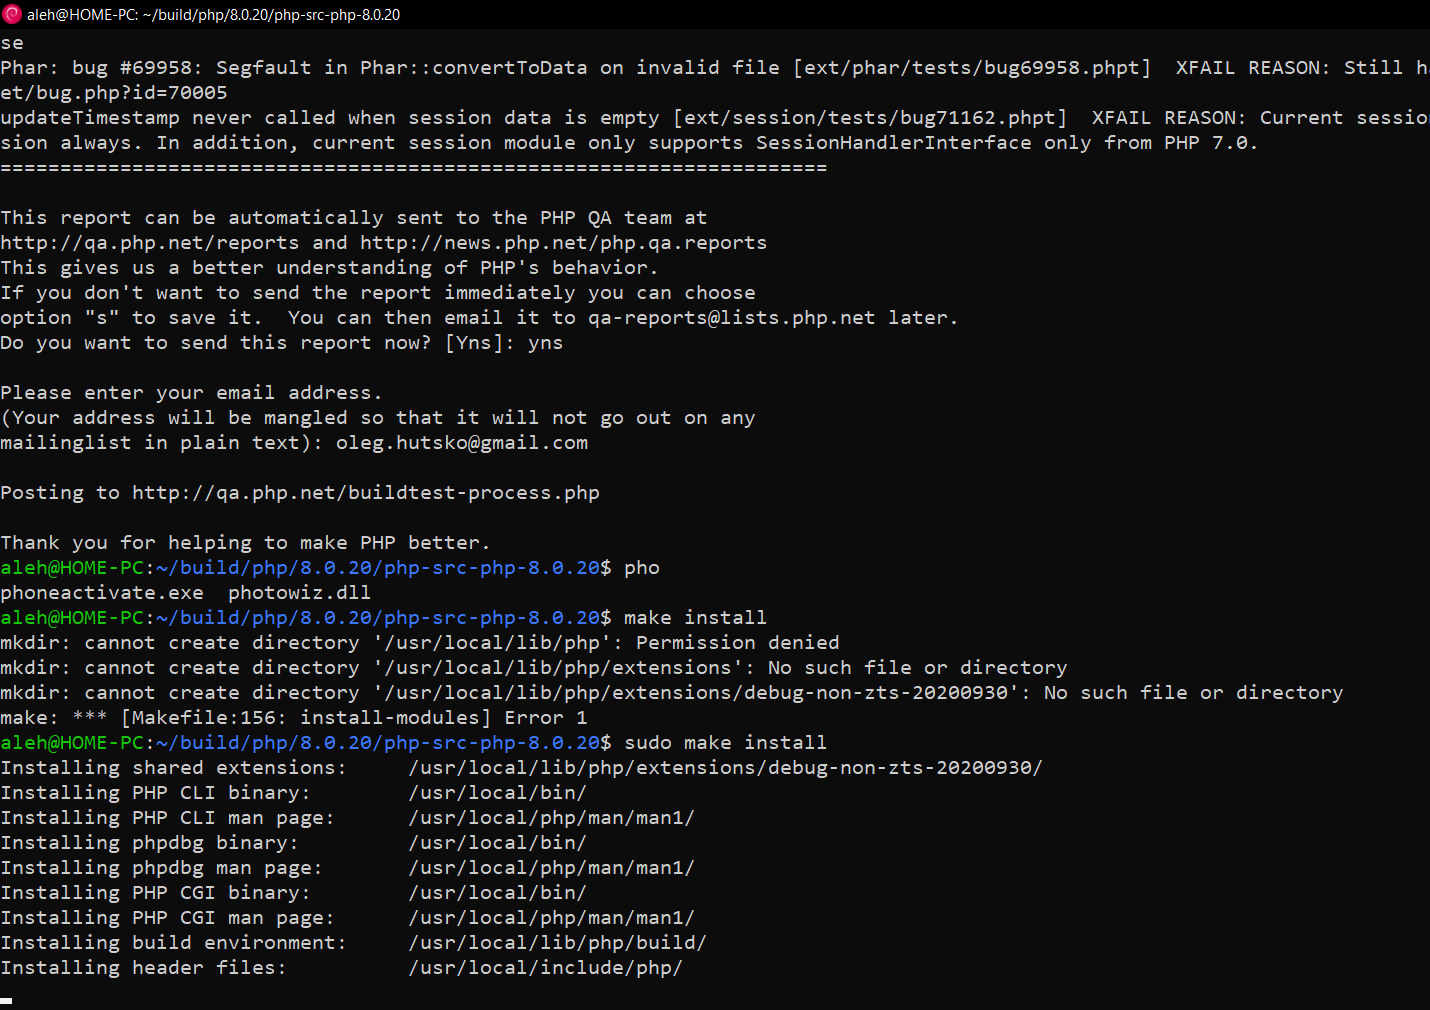
\includegraphics[width=16cm]{e11.png}
	\caption{Koniec "make test", polecenie "sudo make install"}
    \label{fig:sixth}
\end{figure}

\begin{figure}[h]
    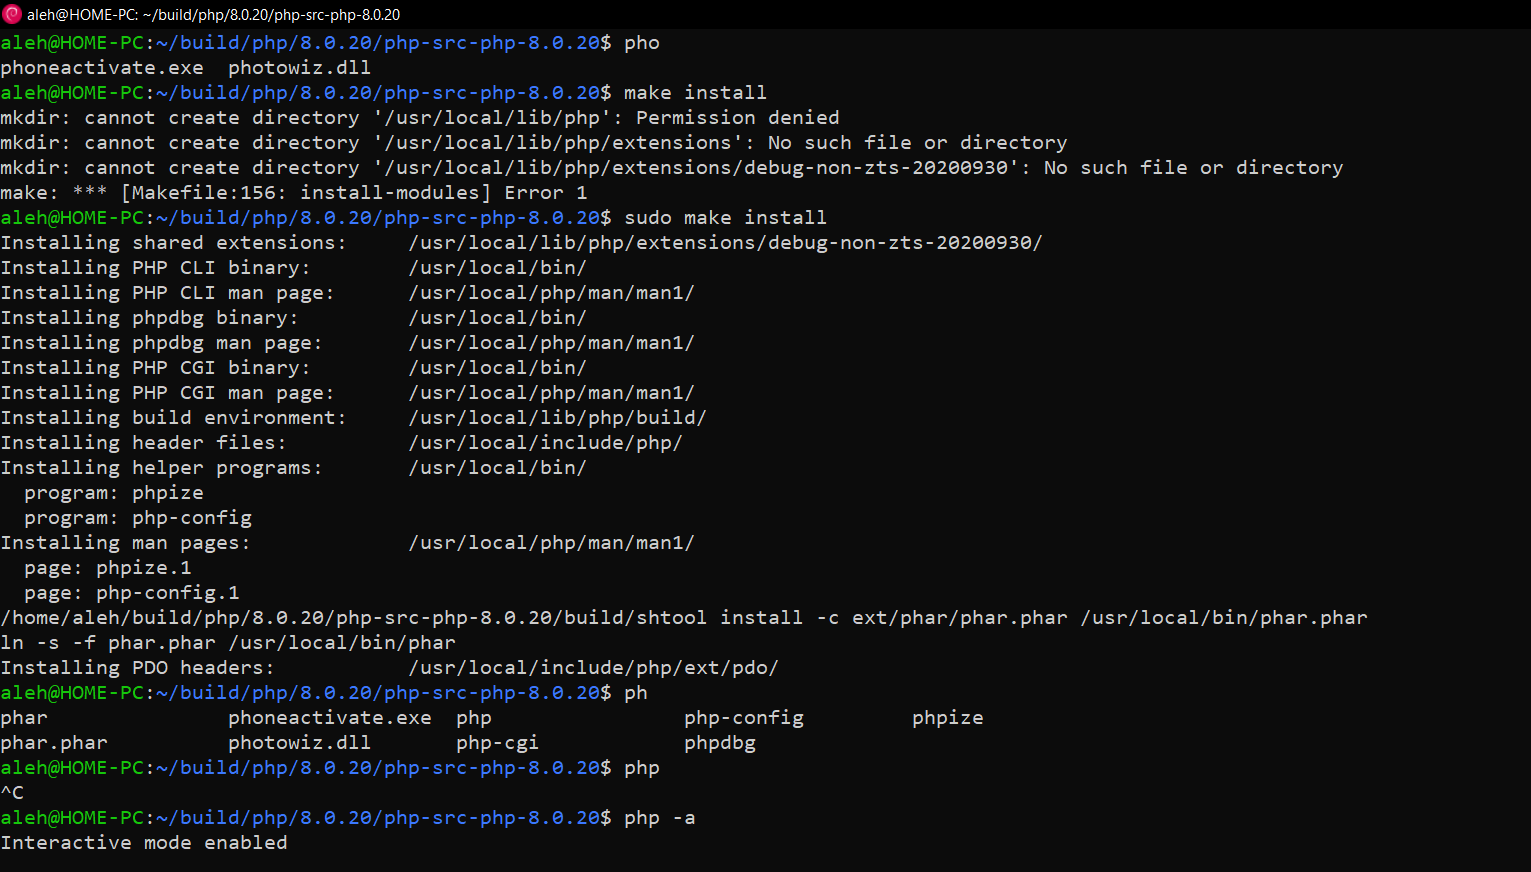
\includegraphics[width=16cm]{e12.png}
	\caption{Koniec "sudo make install"}
    \label{fig:seventh}
\end{figure}

\chapter{Wynik instalacji programu}

\begin{figure}[h]
    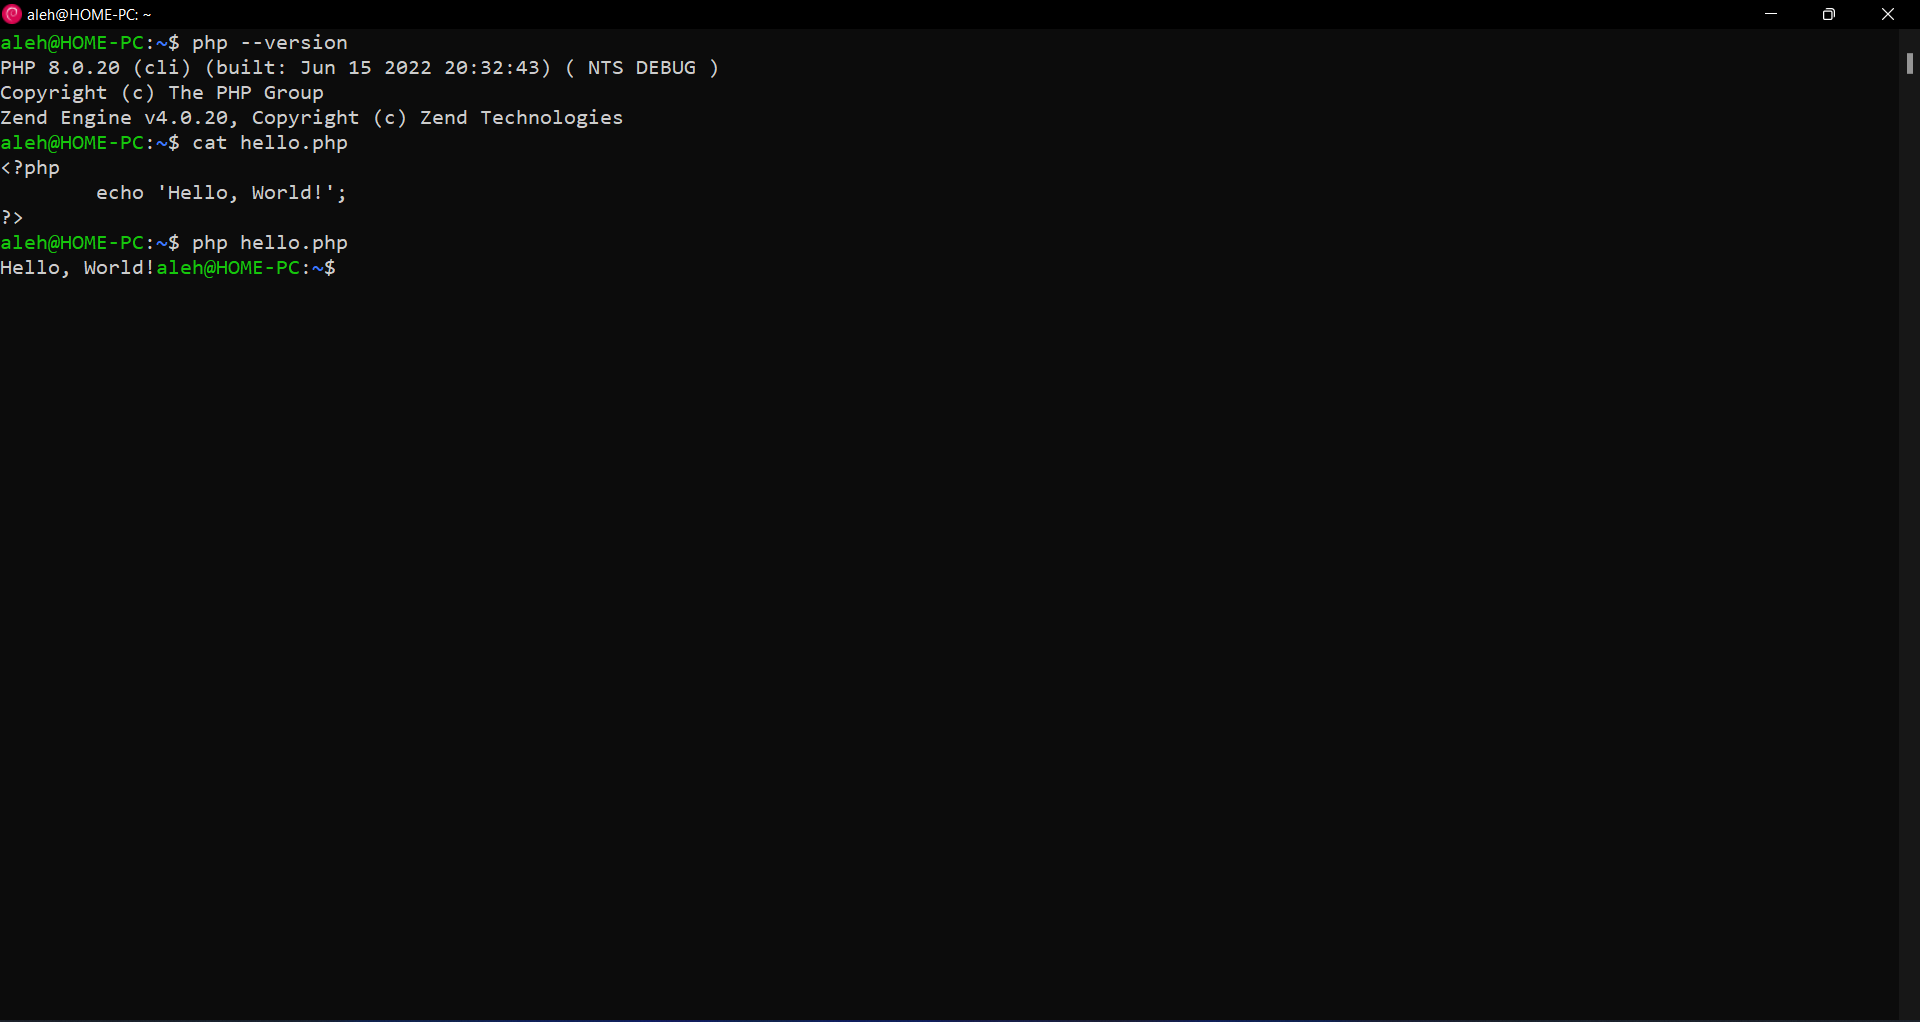
\includegraphics[width=16cm]{workingProgram.png}
	\caption{Sprawdzenie czy php został zainstalowany}
    \label{fig:eight}
\end{figure}

\chapter{Podsumowanie}

Zespół PHP prowadza nam fajną instrukcje po instalowaniu ze źródeł, u mnie wyszło wszystko z pierwzego razu.
Bardzo mi się spodobała instalacja PHP, jest prosta.
\end{document}